\section{Activités en entreprise}

Mes journées dans l'entreprise sont rythmées par l'organisation que je me donne pour accomplir mes projets. J'ai une vision d'ensemble de l'objet final qui m'est donné par mon maître d'apprentissage et son cahier des charges, et je m'organise au mieux pour documenter et fournir un travail estimable de son début à sa toute fin.
\\ \\
Plusieurs projets m'ont été confiés, pour la plupart terminés mais pour ceux les plus récents encore en cours de réalisation.

\subsection{Projets accomplis}

Les projets terminés sont ceux obtenus à mon entrée dans l'entreprise, ceux de moyenne ou de petite taille, ou ceux pour lesquels j'avais une partie des connaissances nécessaires pour les aborder avant de les étudier. J'ai ainsi procédé à différentes activités dans l'entreprise dans l'ordre suivant.

\subsubsection{Montage de services d'administration et de partage de données}

Définie dans ma fiche de poste à mon arrivée dans l'entreprise, était demandée une collection d'applicatifs répondant aux besoins de l'équipe pour faciliter notre travail quotidien. Ceux-ci ne pouvaient être présents auparavant par manque de temps pour les mettre en place, pour les maintenir et pour la montée en compétences de certains domaines abordés.
\\ \\
En voici la liste de solutions que j'ai déployées la première période dans l'entreprise, à l'écoute des besoins de mes collègues et de ma fiche de poste pour faciliter le travail quotidien de l'équipe en interne et envers les clients.

\begin{itemize}
  \item Une \textbf{interface de gestion des applications conteneurisées}
  \item Un \textbf{serveur mandataire d'accès inverse} pour nos services WEB.
  \item Une \textbf{solution de partage de mots de passe sécurisée}.
  \item Une \textbf{plateforme d'échange de fichiers volumineux}.
  \item Une \textbf{console de vérification de la disponibilité de nos sites hébergés}.
  \item Une \textbf{infrastructure de développement et d'échange de code}.
\end{itemize}

\noindent L'intérêt mon travail fut de comprendre au mieux les besoins de mon équipe pour approcher ces solutions en répondant au mieux à leurs besoins, ou d'au moins pouvoir les réorienter vers une ou plusieurs autres optiques de raisonnement. Mon travail fut aussi de mettre en place ces solutions d'une manière sécurisée, documentée et stable.

\paragraph{L'intérêt de l'interfaçage d'applicatifs en équipe}

Les solutions déployées fonctionnent sous forme de micro-services, dit conteneurisés, en utilisant la technologie Docker. Celle-ci permet de réduire l'empreinte des solutions lancées et de facilement pouvoir les maintenir et remanier.% : les redémarrer, les mettre à jour et les réagencer stablement.
% Docker permet un contrôle de version des applicatifs pour facilement revenir sur une ancienne version si les mises à jour sont conflictuelles, une intégration simple avec les autres micro-services, une facilité dans leur déploiement et j'en passe.
\\ \\
L'inconvénient de cette technologie est qu'elle a besoin d'être appréhendée efficacement pour s'en servir correctement car complexe à l'accommodation - possible uniquement en lignes de commande. C'est pour cela que pour aider l'équipe à les maintenir et à appréhender la technologie, j'ai implémenté une interface de gestion de ces micro-services par le suivis d'actions plutôt que par des lignes de commandes.
\\ \\
L'équipe peut désormais profiter de la flexibilité et des fonctionnalités de Docker en utilisant une interface graphique et en lisant des procédures plutôt que d'apprendre les principes, et devoir prendre du temps à prendre en main la technologie.
\\ \\
J'ai appris en entreprise que l'on ne travaille pas pour soit ni seul, mais généralement en équipe et ici pour une équipe. Je pouvais monter les meilleurs services selon moi, mais ceux-ci n'auraient pas été accessibles par l'équipe, ne sachant le raisonnement ou les connaissances que j'avais de la solution.
\\ \\
J'en retiens d'en favoriser l'accessibilité aux fonctionnalités lorsque cela est nécessaire, sur le moment et plus tard lorsqu'une personne devra reprendre le projet (comme ce fut le cas pour moi); en documentant mon travail, en y ajoutant des procédures détaillées et en essayant de favoriser le nécessaire au meilleur si cela complexifie trop le travail - ici de l'apprentissage d'une technologie pour manier des solutions.
% \\ \\
% Au fur et à mesure que je travaillais avec les technologies de l'entreprise et Docker, je me suis plus à en apprendre davantage sur elles.

\paragraph{Le rôle d'un serveur mandataire d'accès inverse en entreprise}

J'ai monté un serveur mandataire d'accès inverse, aussi dit Reverse Proxy, pour héberger les micro-services conteneurisés.
\\ \\
Un serveur mandataire d'accès est un serveur par lequel les utilisateurs sont obligés de demander (mandataire) pour accéder à un ou plusieurs services (serveur d'accès), généralement hébergés sur Internet.
\\ \\
Ainsi, dans les universités ou autres institutions est souvent installé de manière transparente un serveur mandataire d'accès pour limiter l'activité des utilisateurs sur Internet, car bloqué par le serveur d'accès ou pour journaliser leurs activités.
\\ \\
Un serveur mandataire d'accès \underline{inverse} effectue les mêmes opérations mais dans le sens inverse : il laisse les utilisateurs accéder à des ressources, mais journalise leurs activités et permet l'utilisation des services en passant par un point d'entrée unique d'entrée exposé à l'extérieur.
\\ \\
Son intérêt devient crucial en sécurité, amincissant la surface d'attaque possible des sites en faisant circuler les connexions par un seul endroit journalisant les activités.

\begin{figure}[H] % H fixed h flexible
  \centering
  \captionsetup{justification=centering}
  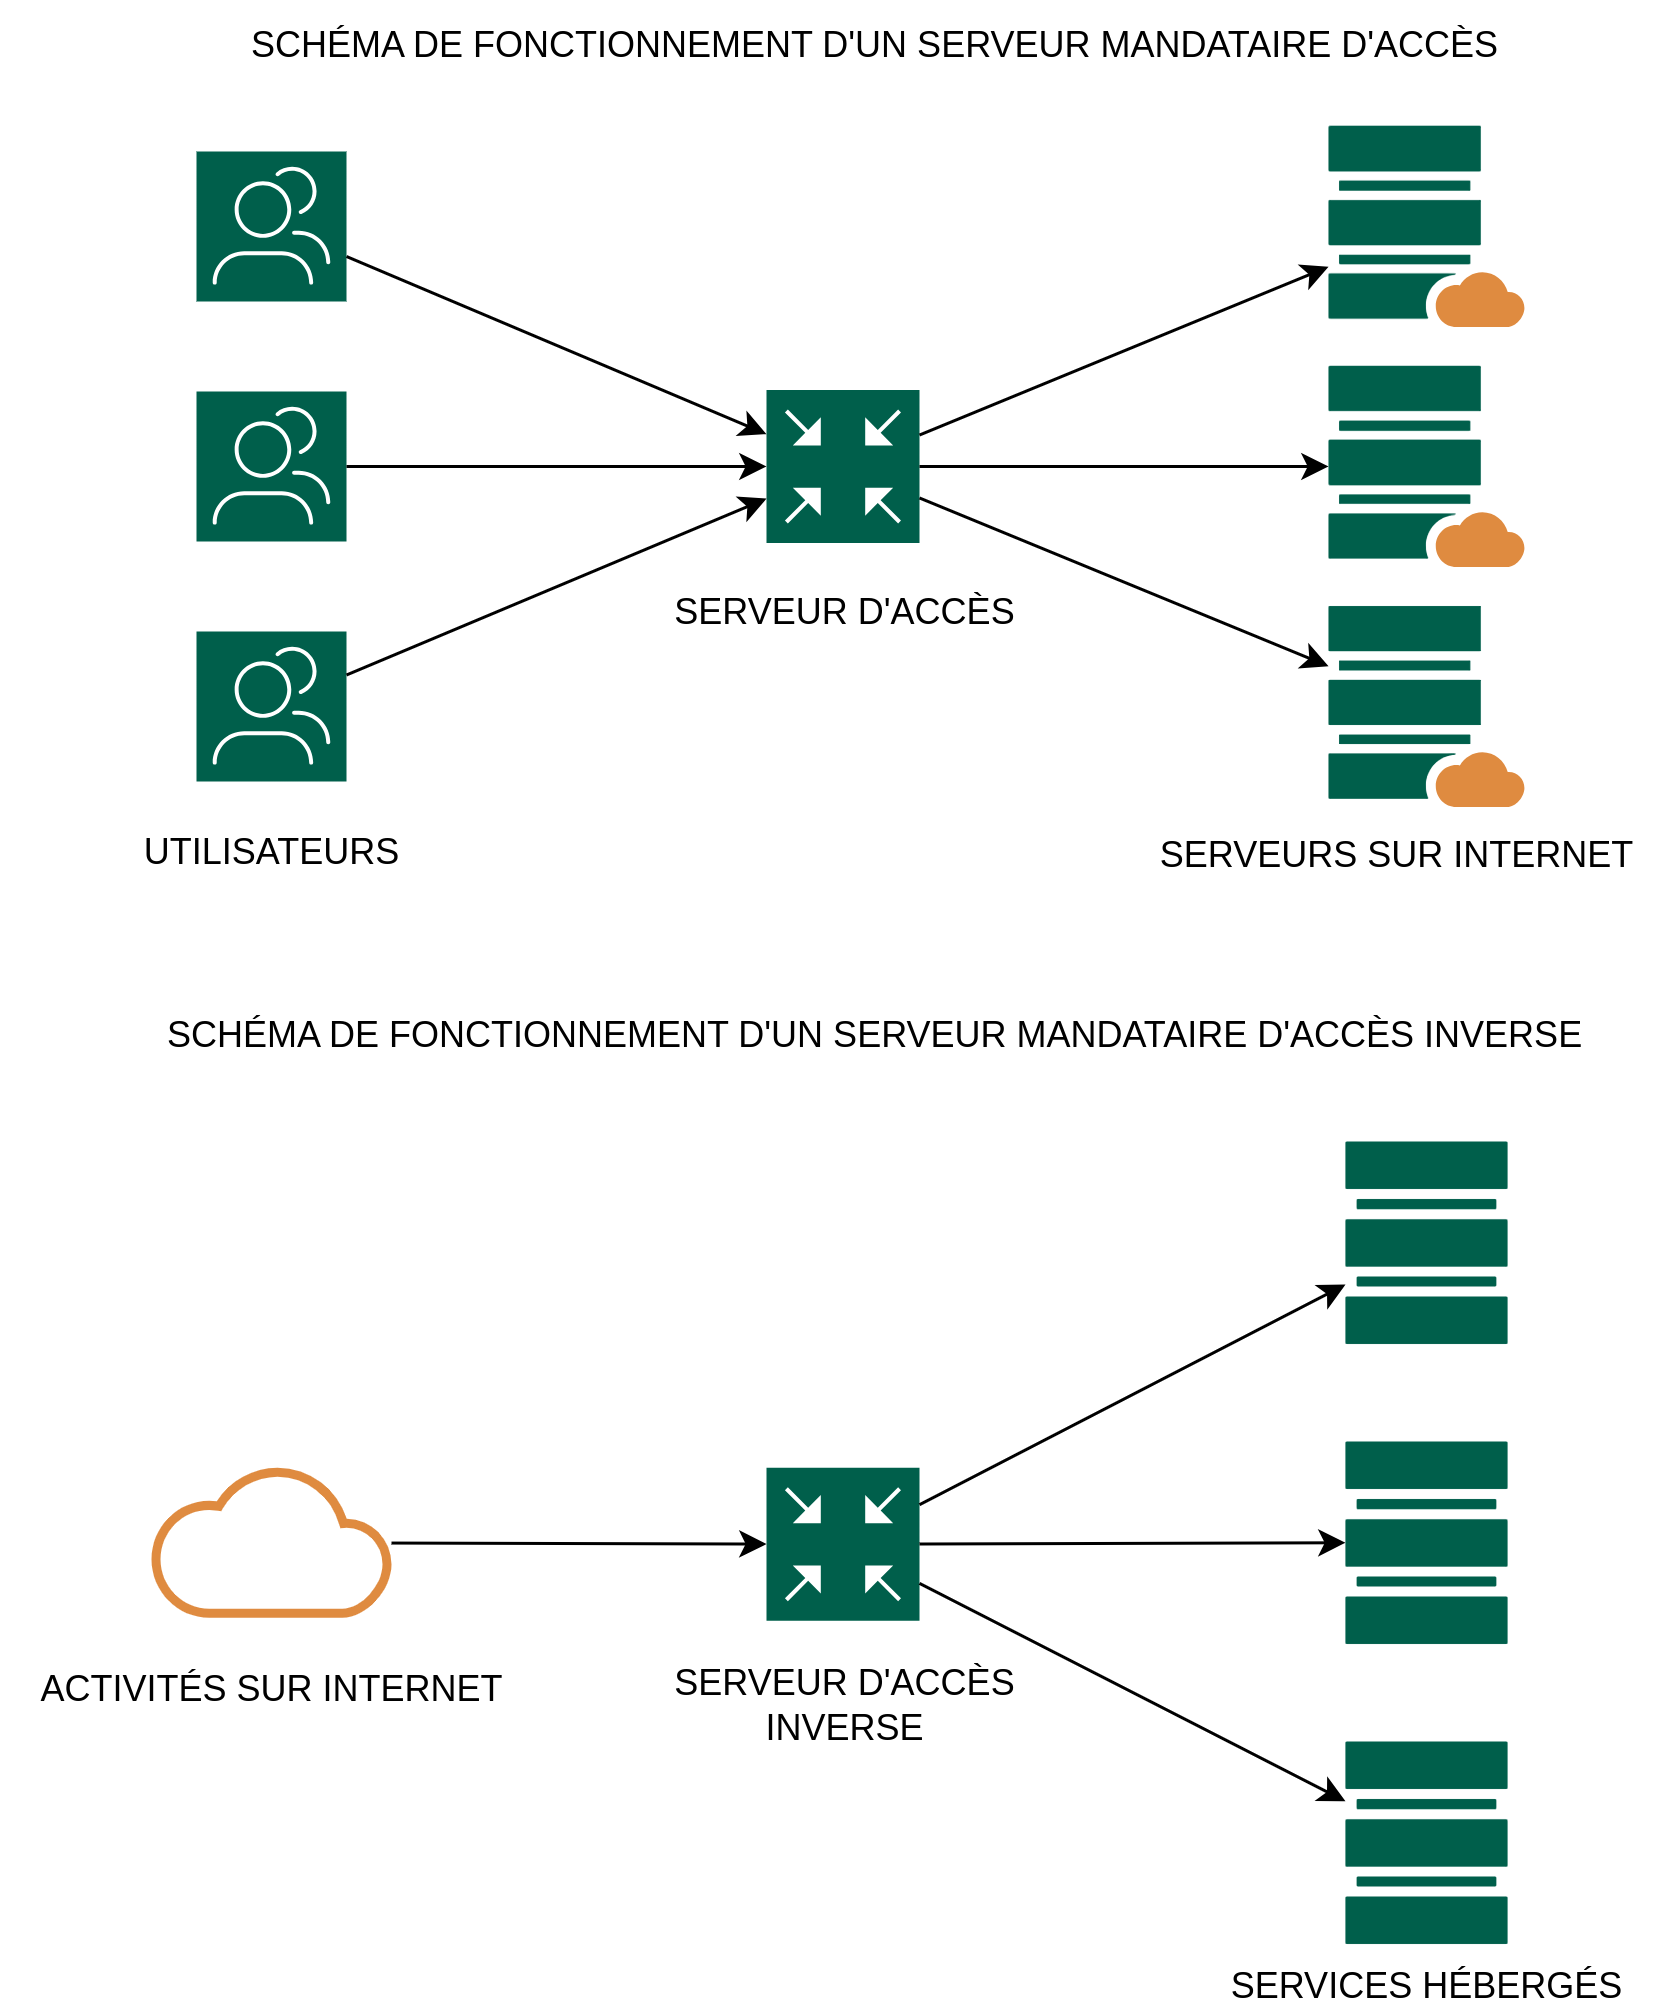
\includegraphics[scale = 0.2]{images/diagrammes/reverse-proxy/serveur_mandataire_acces.png}
  \caption{Schéma de fonctionnement d'un serveur mandataire d'accès et d'un serveur mandataire d'accès inverse.}  
  \label{fig:serveur_mandataire_acces} % pour la citer après
\end{figure}

\noindent J'ai ainsi monté un serveur mandataire d'accès inverse pour les solutions hébergées en micro-services, lui-même dans un micro-service. En résultant une exposition contrôlée des solutions hébergées et accessibles depuis l'extérieur, notamment par nos clients.

\paragraph{Découverte de l'importance d'échanger les mots de passe de manière chiffrée avec les clients}

% à modif
Lors de mon arrivée dans l'entreprise, j'ai remarqué qu'il n'y avait pas de politique d'échange de mots de passe avec les clients. Certaines personnes de l'équipe envoyaient les mots de passe en texte par courriel, d'autres par des liens de services dédiés pour faire accéder aux clients leurs mots de passe sans le divulguer explicitement dans les courriels.
\\ \\
Je me suis aussi rendu compte que, parce que non initiés aux bonnes pratiques, nos clients utilisent souvent des mots de passe faillibles.

\subsubsection{Étude et mise en production d'une nouvelle solution de support client}

ADITU possède trois moyens de communication avec ses clients : les courriels, les échanges téléphoniques et une solution de support en ligne. Par la dernière, les clients ouvrent peuvent ouvrir un ticket pour une demande ou un problème qu'ils rencontrent et s'assurent d'un suivi clair et pérenne de leur démarche à un seul endroit.
\\ \\
Cette dernière était cependant la moins utilisée, nos clients la trouvant la plus vieillissante, la plus simpliste et la moins agréable visuellement et à l’utilisation. De notre côté, l'équipe se plaignait du manque de praticité pour la gestion des tickets et d’une trop faible flexibilité dans son utilisation (impossible de faire du cas par cas).
\\ \\
Projet majeur de cette première année d'alternance, mon travail fut de rechercher une nouvelle solution professionnelle de support client en élaborant une étude comparative et budgétaire des solutions disponibles sur le marché, pour les étudier comportementalement en environnement contrôlé m'assurer qu'elles répondaient au mieux à nos besoins dans leur utilisation; pour effectuer la mise en production de la solution retenue et vérifier sa bonne utilisation et de la compréhension des clients.
\\ \\
Projet fil rouge de mon alternance, l'ensemble des manipulations me demandaient du sens et de la rigueur. L'étude comparative et les mises en situation furent longues et intéressantes. J'y ai appris que lors d'une étude comparative, il fallait davantage comparer les solutions sur les besoins auxquelles elles répondaient plutôt que sur les fonctionnalités qu'elles proposaient.
\\ \\
En effet, nous ne voulions pas choisir la meilleure solution mais celle qui répondait au mieux à nos besoins. Ainsi, j'ai pris l'initiative de noter les solution de 0 à 3 sur la qualité de leur réponse au cahier des charges que je m'étais fixé, dont en voici le résultat.

\begin{table}[H]
    \centering
    \captionsetup{justification=centering}
    \begin{tabular}{|l|l|l|}
    \hline
    Réponse au cahier des charge par les solutions            & Combodo iTop & Teclib' GLPI \\ \hline
    Ticketing                                                 & 3            & 3            \\
    Devis et Facturations                                     & 3            & 0            \\
    Front-end client et Back-end admin                        & 3            & 2            \\
    Création d'incidents                                      & 2            & 2            \\
    Demandes de changements par les utilisateurs              & 3            & 2            \\
    Création de tickets automatique                           & 3            & 3            \\
    Suivi des modifications des demandes                      & 3            & 3            \\
    Connecteur OCS pour informations                          & 3            & 3            \\
    Tableau de bord personnalisable                           & 3            & 2            \\
    Fermeture automatique de tickets                          & 2            & 3            \\
    Intégration de la charte graphique de Aditu               & 2            & 2            \\
    Récupération des tickets de vTiger                        & 2            & 2            \\
    Gestion des baies et racks du datacenter (CMDB)           & 3            & 3            \\
    Ouverture de ticket par envoi de mail                     & 3            & 3            \\
    Gestion des ressources (certificats, noms de domaine...)  & 3            & 3            \\
    KB/FAQ                                                    & 3            & 2            \\
    Envoi de mails sur l'information d'activité d'une demande & 3            & 3            \\
    Ajout d'informations individuelles sur le portail client  & 3            & 1            \\
    Gérer les lieux des clients                               & 3            & 3            \\ \hline
    Score total (sur 57)                                      & 51           & 45           \\
    \hline
    \end{tabular}
    \caption{Tableau comparatif des solutions conservées après les études en environnement contrôlé.}
    \label{tab:comparatif} 
\end{table}

\noindent S'en est suivi l'installation dans un milieu de production et la documentation de mes démarches pour son installation. J'en ai appris que lors d'un travail en équipe, il était crucial de maintenir ses efforts à l'explication des principes et des découverte, choses non primordiales lors d'un travail individuel non amené à être partagé.
\\ \\
En parallèle ont été envoyés, parfois avec mon tuteur, des courriels de rappel du changement de l'interface de support à nos clients. Ainsi, nous conservions un contact avec eux et nous ne les prenions pas au dépourvu le jour du changement. Tous les tickets de l'ancienne interface étaient disponibles sur la nouvelle interface le jour de la bascule, une documentation d'utilisation leur a aussi été délivrée.
\\ \\
Avec beaucoup de préparation et du temps, l'installation et le déploiement s'est passé sans encombrement majeur, je relate cependant quatre points d'amélioration que je m'efforcerai de ne pas reproduire.

\begin{itemize}
  \item Ne pas avoir fait d'\underline{environnement de développement} une fois la solution mise en place. Faire des modifications directement sur l'interface utilisée par les clients n'est pas une bonne chose à faire et je le reconnais maintenant, même en connaissant bien la solution. J'ai donc monté à l'identique l'interface en interne pour tester les modifications avant qu'elles ne soient déployées sur l'interface utilisée par les clients, afin de prévenir d'impacter l'environnement actif et éviter d'éventuels problèmes liés aux changements. 
  \item Avoir utilisé des \underline{mots de passe trop complexes pour les clients}. J’ai préféré générer un mot de passe aléatoire et complexe pour chaque client à leur première connexion. Question sécurité, cela me paraissait être une bonne pratique. Question practicité, c’était infâme pour les personnes novices en informatique qui appelaient car n'arrivant pas à se connecter en recopiant leur mot de passe manuellement à cause de caractèers spéciaux et/ou non usuels. Désormais, je m'éfforce de générer des passphrases avec des informations simples remaniées avec des caractères spéciaux usuels.
  \item Dans mon processus de distribution des identifiants, au lieu de transférer les mots de passe par courriel, j’indiquais que ceux-ci était accessibles en suivant un lien. Ce qui évite si la boite mail d’un client est compromise qu'un attaquant puisse les essayer ailleurs. Cependant, certains clients comprenaient que leur mot de passe était ce lien, et le recopiait dans le champ attendu pour leur mot de passe. L’histoire du \underline{"lien vers le mot de passe" plutôt que le mot de passe}... La prochaine fois que je communiquerai des informations de connexion ou d’identification, je ferai en sorte d’attirer le regard du destinataire vers des lignes précisant le plus simplement possible comment accéder à leur mot de passe, en cliquant d'abord sur le lien.
  \item Pour le renseignement des tickets, les clients passent par une suite d’étiquettes pour leur faciliter l’accommodation avec l’interface. Ils ont premièrement deux choix : "Demande" ou "Incident", puis ils précisent un service impacté ("Messagerie", "Sauvegarde"...). Le problème remonté par un client était qu'il trouvait que les noms ne lui faisaient pas sens, et j'ai ainsi compris qu'\underline{il faut utiliser les mots qui font le plus de sens aux clients} plutôt que ceux qui nous semble les plus justes. Lorsque je communique avec les clients désormais, je m’efforce d’expliquer les choses avec leurs mots plutôt que les miens, même si ceux que j’utilise sont les plus appropriés ou justes : l'explication est faite au client, pas à moi - je me dois d'utiliser des explications les plus proches de sa compréhension initiale.
\end{itemize}

Lors de cette activité, j'ai appris à effectuer une étude comparative correcte et à synthétiser mon travail pour faire part de mes apprentissages intéressants aux autres membres de l'équipe. J'ai aussi appris de mes erreurs vis-à-vis des relations clients (mots de passe, liens, séparer l'environnement de modifications de celui en production...)
\\ \\
En résultant, l'interface de support d'ADITU est nouvelle et accueillante, bien plus pratique à l'utilisation au quotidien pour les clients et l'équipe technique.

\subsubsection{Procédure d'assainissement et de mise à jour d'équipements actifs}

% à modifier

\underline{\textbf{je préfère attendre les premiers retours pour commencer à rédiger}}
\underline{\textbf{pour ne pas faire fausse route dès le départ et perdre du temps}}

% fin à modifier

\subsection{Activités en cours de réalisation}

J'apprends beaucoup des activités non terminées en cette fin de première année. Ceux-ci regroupent d'autres projets imposants à criticité importante, faisant appel ce que j'ai pu découvrir et apprendre, mais aussi à des compétences que je n'ai pas encore.

\subsubsection{Réagencement du système d'accès administrateur}

Pour gérer les connexions à leurs machines, les administrateurs systèmes essayent généralement d'avoir à retenir le moins de mots de passe possible. Au contraire, nous préférons utiliser un gestionnaire de mots de passe ou un système de clés, comme sur des maisons : au lieu de retenir un digicode pour chaque porte, nous mettons une serrure et nous nous assurons qu'uniquement nous possédions la clé.
\\ \\
Le système de clés pour les connexions à distance est souvent le plus privilégié : rapide, robuste et permettant l'authentification des personnes utilisant leurs clés. Cependant, dans son utilisation celui-ci peut devenir faillible : si la même clé est utilisée pour toutes les serrures, pareil si c'était un digicode, une personne récupérant ou ayant une copie de cette clé pourrait déverrouiller toutes les portes.
\\ \\
Par cette analogie, je viens d'expliquer le fonctionnement du système de connexion aux machines distantes qu'avait ADITU. Par souci de facilité, au début de l'entreprise une personne avait l'habitude d'enregistrer sa clé sur les équipements, que les autres membres de l'équipe s'accaparait aussi; et ainsi, tout le monde utilisait finalement la même clé.
\\ \\
Autre problème de cette méthode : on ne sait pas qui s'est connecté en utilisant cette clé et s'il en avait le droit. Car normalement, chacun possède sa clé universelle lui permettant d'accéder aux endroits qu'il devrait avoir accès : si tout le monde a la même clé, tout le monde a accès à l'ensemble du parc.
\\ \\
Autrement dit, si une ancienne personne de l'entreprise ou un attaquant arrivait à se procurer la dite clé : il aurait accès à l'ensemble des machines d'ADITU.
\\ \\
Une première initiative que j'avais eu fut d'avoir fait générer une clé (informatique) individuelle à chaque membre de l'équipe et de laisser Guillaume, notre Directeur technique, décider des machines auxquelles les membres devraient pouvoir accéder - sécurisation du système d'accès à distance (limiter l'exposition de nos machines si une clé venait à être dérobée).
\\ \\
Problème de cette solution, pour chaque personne devant accéder à une nouvelle machine, une personne déjà en accès sur celle-ci devait manuellement lui créer une serrure. Cette solution était piètre dans notre service et c'est pour cela que je ne l'ai pas instaurée, chacun devant aussi accéder à toutes les serrures à un moment ou à un autre en urgence ou non. Mais cette réflexion reste extrêmement importante du point de vue sécuritaire des accès.
\\ \\
Ainsi, pour répondre à cette problématique, j'ai décidé d'instaurer une machine dite bastion pour éviter de gérer manuellement l'accès aux machines à la main. Ainsi peuvent être gérés les accès par groupes de machines, d'utilisateurs et pour une durée limitée simplement. 

\begin{figure}[H] % H fixed h flexible
  \centering
  \captionsetup{justification=centering}
  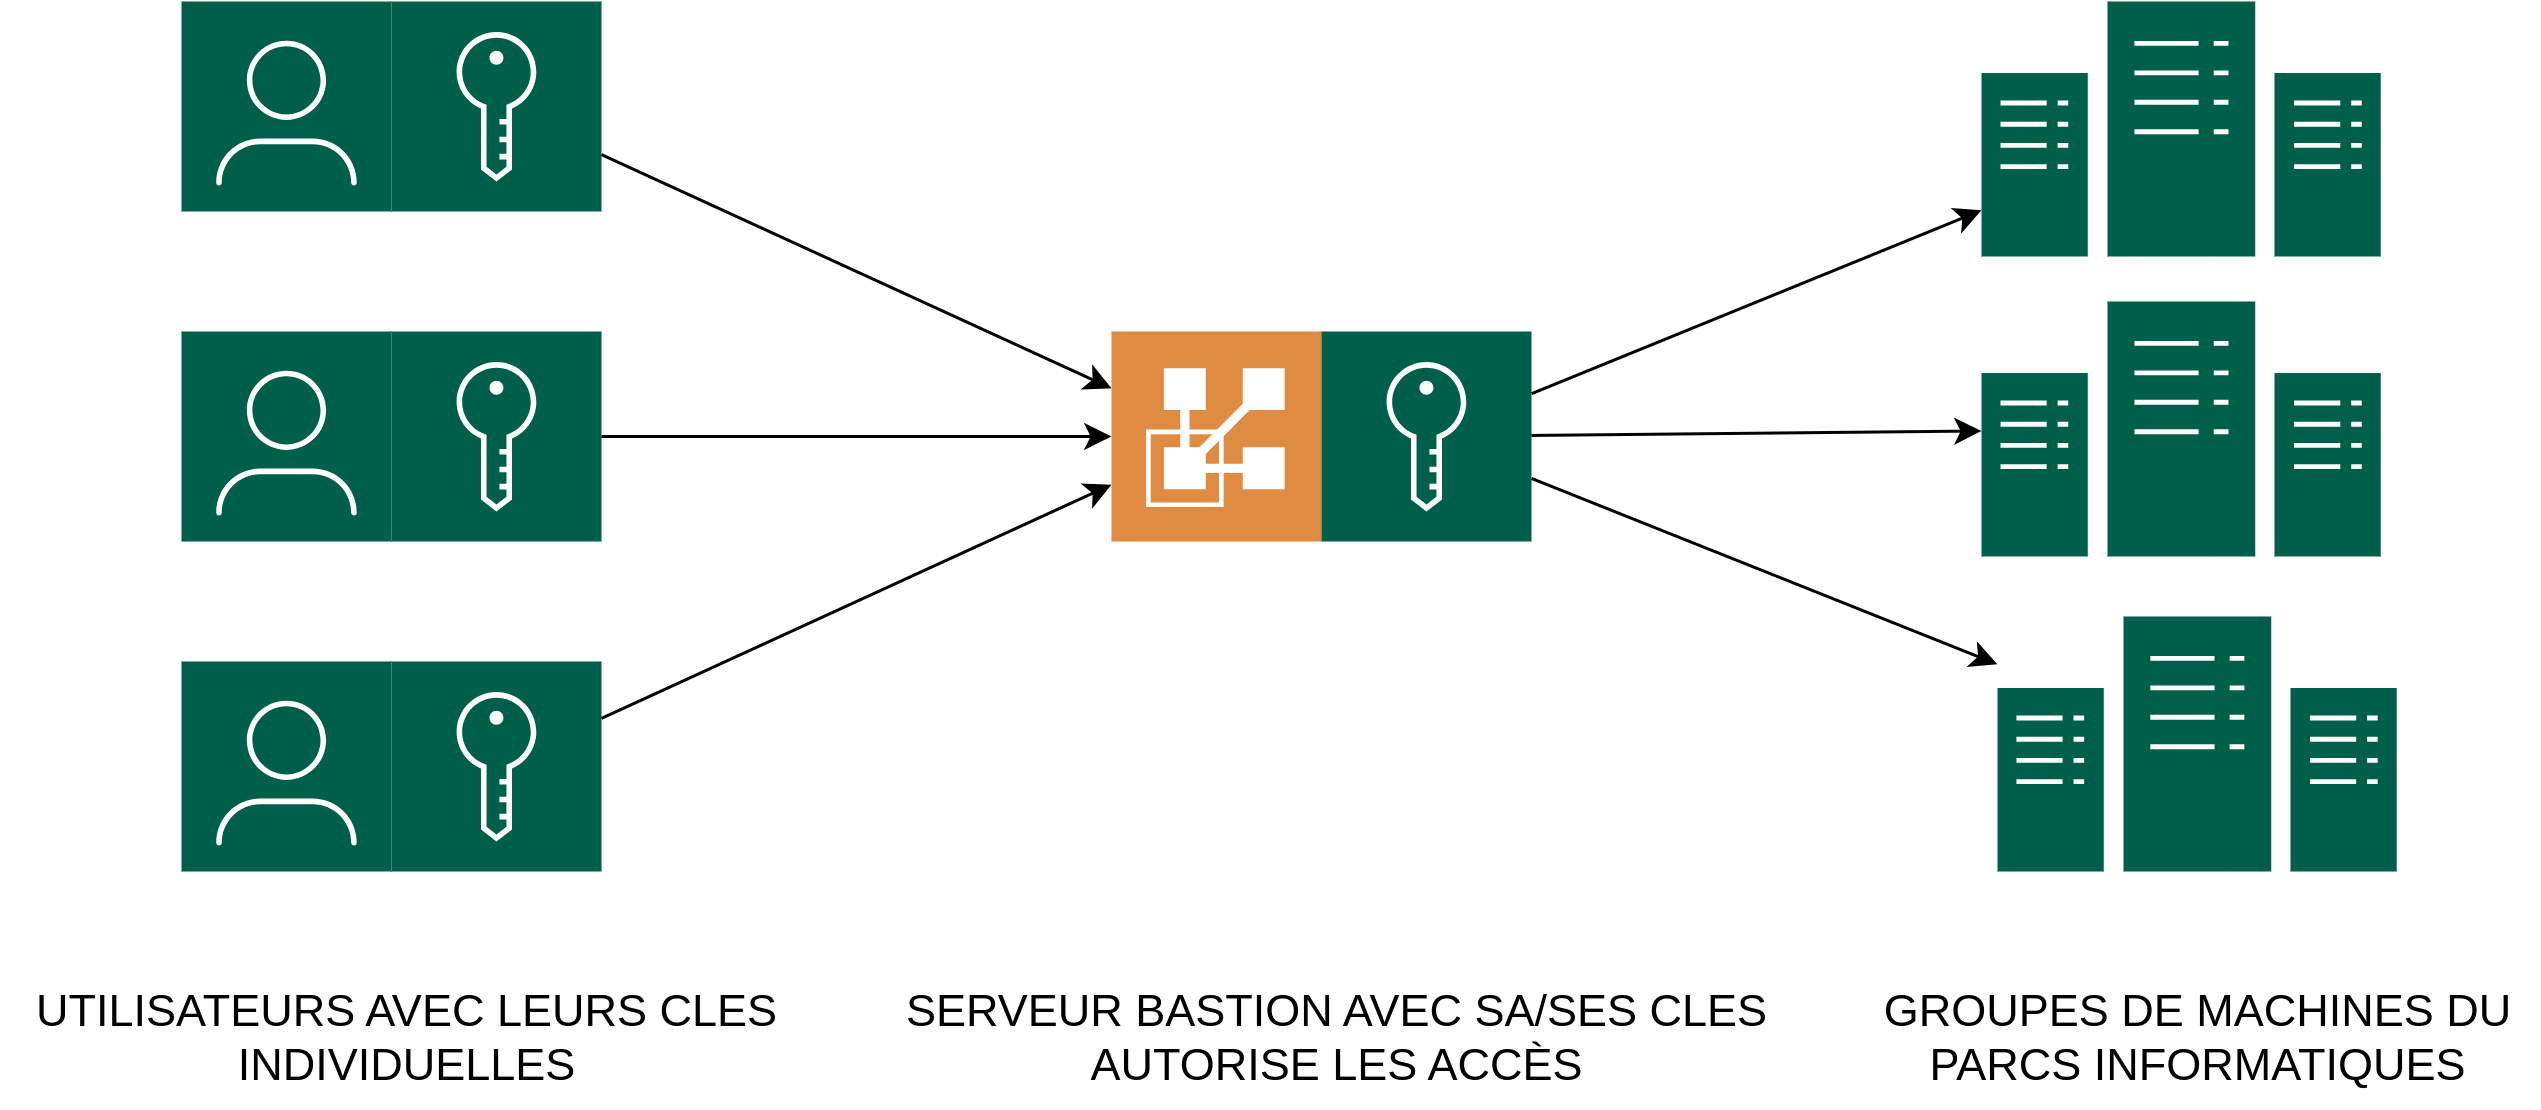
\includegraphics[scale = 0.15]{images/diagrammes/bastion/bastion.png}
  \caption{Utilisateurs accédant à distance à leurs parcs informatiques avec une machine bastion. Les utilisateurs s'authentifient avec leur clé auprès du bastion, qui contrôle et autorise les accès aux machines. Aucune personne n'est en connaissance ou en capacité de récupérer la/les clés du bastion.}  
  \label{fig:bastion} % pour la citer après
\end{figure}

\noindent J'ai donc commencé l'étude pour le choix d'une solution pour un serveur bastion, de son implémentation et de son maintient.
\\ \\
J'apprécie ce rapport à la sécurité dans cet exercice en cours de complétion. Celui-ci me permettra de renforcer mes compétences en sécurité et celles d'ADITU, en ségmentarisant les accès des machines aux personnes en ayant uniquement l'autorisation, et ce plus facilement. Répondant au problème initial de l'accès ouvert à tous, et à celui découvert de maintenir ce niveau de sécurité élevé.

\subsubsection{Conceptualisation et intégration d'une nouvelle solution de supervision}

\underline{\textbf{je préfère attendre les premiers retours pour commencer à rédiger}}
\underline{\textbf{pour ne pas faire fausse route dès le départ et prendre du temps}}

\subsubsection{Réorganisation des réseaux privés virtuels des réseaux d'un data centre}

\subsection{Activités annexes}

D'autres activités m'ont permis une montée en compétences et de mieux accomoder le monde de l'entreprise : la prise de séances de formation et les sorties.

\subsubsection{Suivi de séances de formation}

\textit{pourquoi j'avais besoin de formations + dire qu'au début je ne voyais pas pourquoi (j'ai appris : que je pouvais y assister pour aider les autres)}
\\
\textit{organisation des formations dans la semaine, dans quel but initial}
\\
\textit{ce que cela m'a apporté, pourquoi ça m'a aidé (explications, voir une vision différente d'une même notion)}

\subsubsection{Déplacements sur sites et en clientèle}

\textit{pourquoi j'ai eu besoin de me déplacer : la raison à chaque fois, pour apprendre}
\\ \\
\textit{déplacements sur site client pour de l'installation où j'ai aidé (soliha), et à dax pour apprendre et visualiser}
\\ \\
\textit{répondre à : est-ce que j'ai envie d'en refaire, est-ce que la clientèle m'intéresse}

\subsection{Bilan horaire et de compétences}

\textit{ici un diagramme de gantt de mes semaines pour montrer sur chacune des 29 semaines chez ADITU sur quoi j'étais (les services montés, puis sur iTop mais d'autres choses en parallèle...) pour leur donner le temps}
\\ \\
\textit{je mettrai aussi un diagramme camembert des domaines que j'ai touché, le quoi\\
réseaux 30\%
\\
développement et étude 25\%
\\
administration 20\%
\\
sécurité 10\%
\\
déplacements 10\%
\\
formations 5\%}

\newpage